%%%%%%%%%%%%%%%%%%%%%%%%%%%%%%%%%%%%%%%%%%%%%%%%%%%%%%%%%%%%%%%%%%%%%%
% Problem statement
\begin{statement}[
  problempoints=100,
  timelimit=1 second,
  memorylimit=1024 MiB,
]{Sirologija}

You are an ant, but not just any ant – you're an ant obsessed with cheeseology!

You've discovered a new slice of cheese in the kitchen and want to send as many of your minions as possible to explore it. Imagine the cheese as a table with $N$ rows and $M$ columns, where the rows are labeled from $1$ to $N$ from top to bottom, and the columns are labeled from $1$ to $M$ from left to right. Some fields contain holes, while others contain cheese. We will denote the field in the $r$-th row and $s$-th column as $(r, s)$. The top-left and bottom-right fields will definitely contain cheese.

Let's denote the number of minions as $K$. Your minions will start their exploration in the top-left field and finish in the bottom-right field. They can only move downwards and to the right. Additionally, their paths must not "cross", meaning we can assign labels from $1$ to $K$ to them in such a way that there is no field from which a minion with a lower label exited to the right, and a minion with a higher label exited downwards.

Moreover, you would like these paths to be "different" in some sense, meaning that for every two minions, there exists a field $(r, s)$ containing a hole, such that one of them was at some point in column $s$ and in a row labeled lower than $r$, while the other was at some point (not necessarily simultaneously) in column $s$ and in a row labeled higher than $r$. Informally, every pair of minions approached some hole from different sides.

Output the maximum value of $K$ such that there exists a selection of minion paths satisfying the given conditions.

Some examples of paths that do not satisfy the conditions:

\begin{figure}[!h]
    \centering
    \begin{subfigure}{0.49\linewidth}
      \centering
      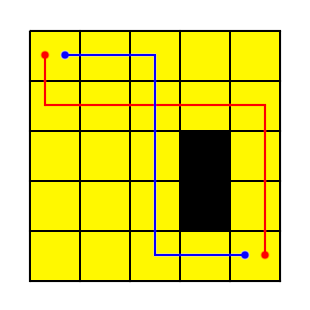
\includegraphics[width=\linewidth]{pic/sijeku_se.png}
      \caption{Invalid choice of paths - they intersect}

    \end{subfigure}
    \begin{subfigure}{0.49\linewidth}
      \centering
      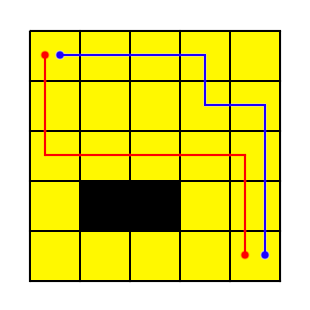
\includegraphics[width=\linewidth]{pic/ista_strana.png}
      \caption{Invalid choice of paths - they approach a hole from the same side}

    \end{subfigure}

  \end{figure}

%%%%%%%%%%%%%%%%%%%%%%%%%%%%%%%%%%%%%%%%%%%%%%%%%%%%%%%%%%%%%%%%%%%%%%
% Input
\subsection*{Input}

The first line contains positive integers $N$, $M$.

The next $N$ lines contain descriptions of the table rows. The $i$-th line contains $M$ characters, where $\texttt{.}$ denotes cheese and $\texttt{\#}$ denotes a field containing a hole.

%%%%%%%%%%%%%%%%%%%%%%%%%%%%%%%%%%%%%%%%%%%%%%%%%%%%%%%%%%%%%%%%%%%%%%
% Output
\subsection*{Output}

Output the maximum possible value of the number $K$ in a single line.

%%%%%%%%%%%%%%%%%%%%%%%%%%%%%%%%%%%%%%%%%%%%%%%%%%%%%%%%%%%%%%%%%%%%%%
% Scoring
\subsection*{Scoring}

In all subtasks, $2 \leq N, M \leq 2000$.

{\renewcommand{\arraystretch}{1.4}
  \setlength{\tabcolsep}{6pt}
  \begin{tabular}{ccl}
   Subtask & Score & Constraints \\ \midrule
    1 & 15 & All holes are in the same row. \\
    2 & 18 & $N, M \leq 10$ \\
    3 & 16 & $N, M \leq 50$, there are no holes in the first or last row or in the first or last column.\\
    4 & 18 & $N, M \leq 50$ \\
    5 & 16 & $N, M \leq 2000$, there are no holes in the first or last row or in the first or last column.\\
    6 & 17 & No additional constraints. \\
\end{tabular}}

%%%%%%%%%%%%%%%%%%%%%%%%%%%%%%%%%%%%%%%%%%%%%%%%%%%%%%%%%%%%%%%%%%%%%%
% Examples
\subsection*{Examples}
\begin{tabularx}{\textwidth}{X'X'X}
\sampleinputs{test/sirologija.dummy.in.1}{test/sirologija.dummy.out.1} &
\sampleinputs{test/sirologija.dummy.in.2}{test/sirologija.dummy.out.2} &
\sampleinputs{test/sirologija.dummy.in.3}{test/sirologija.dummy.out.3}
\end{tabularx}

\textbf{Explanation of the first and second example:}\\

\begin{figure}[!h]
    \centering
    \begin{subfigure}{0.40\linewidth}
      \centering
      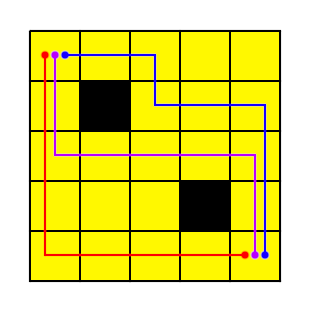
\includegraphics[width=\linewidth]{pic/sir.png}
      \caption{Example of paths for the first sample}

    \end{subfigure}
    \begin{subfigure}{0.40\linewidth}
      \centering
      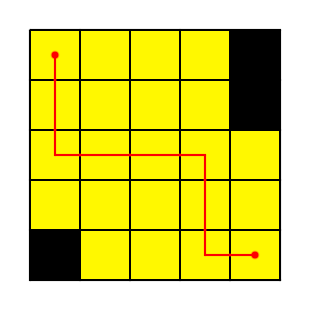
\includegraphics[width=\linewidth]{pic/sir2.png}
      \caption{Example of paths for the second sample}

    \end{subfigure}

  \end{figure}
  
%%%%%%%%%%%%%%%%%%%%%%%%%%%%%%%%%%%%%%%%%%%%%%%%%%%%%%%%%%%%%%%%%%%%%%
% We're done
\end{statement}
